\section{Topic Dynamics of Tweets and News}
\label{sec:top}

In this section, we mainly examine the interaction between news topics and tweets topics by comparing topic dynamics based on the results by \stlda. The interaction between news and tweets is complicated, especially considering the geographic difference in reaction to events.~\newcite{he2015uncovering} find that users in different geographic areas tend to focus differently on an event. In our study, we separate tweets according to geographic boundary of \stlouis where the Ferguson unrest took place. It is assumed that people participating, witnessing or living in nearby areas may behave differently, as reporters, participants or victims. Meanwhile users out of Ferguson area are far away from the place where the event took place, so their knowledge about the event mainly comes from news, social media and other indirect report of the event. The perception of event can be different from people who are experiencing the event. First, we compare topic dynamics in and out of Ferguson area, identifying what the differences are. Second, we compare topics in news and tweets to see whether public opinions are heavily influenced by the media. Specifically, we focus on the overlapping topics in news and tweets, examining the relation between topics of news and tweets.

\subsection{Tweet Topic Dynamics in and out of \stlouis Area}
\label{subsec:tweet_topic}

The topic dynamics of tweets in and out of \stlouis are shown in Figure~\ref{fig:tweets_topics_stlouis}. Under the common topic frame with news, both tweets in \stlouis area and out of \stlouis area lack some topics that only exist in news, thus topic 0 \emph{Obama Talk}, topic 7 \emph{Shoot Accident} and topic 9 \emph{Race and Community}. For the rest topics, it is obvious that topic change is different for tweets in \stlouis area and out of \stlouis.

\begin{figure*}[htpb]
\centering
\subfigure[In \stlouis]
{
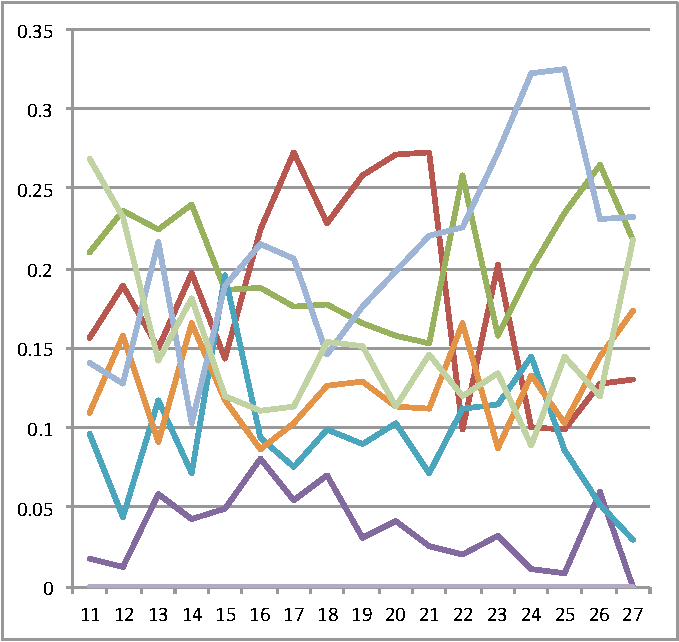
\includegraphics[width=0.48\linewidth]{figures/3LDA2TweetsInSt.pdf}
\label{fig:tweets_topics_inst}
}
\subfigure[Out of \stlouis]
{
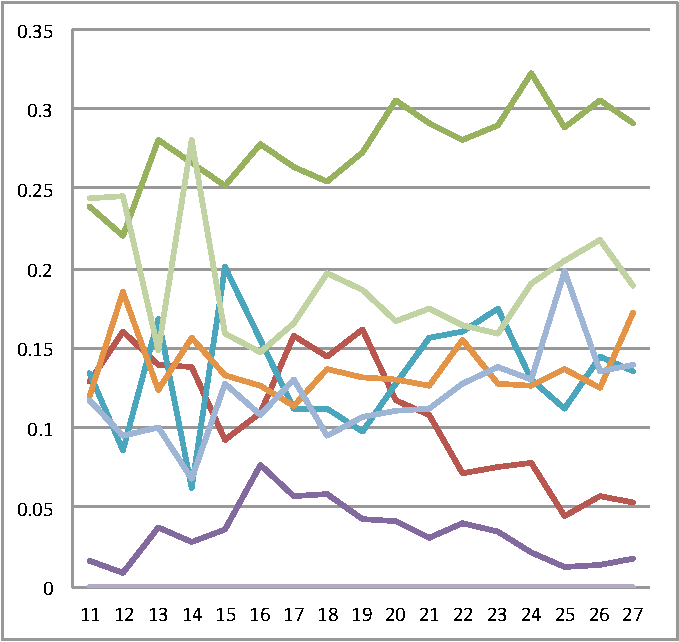
\includegraphics[width=0.48\linewidth]{figures/3LDA2TweetsOutSt.pdf}
\label{fig:tweets_topics_outst}
}
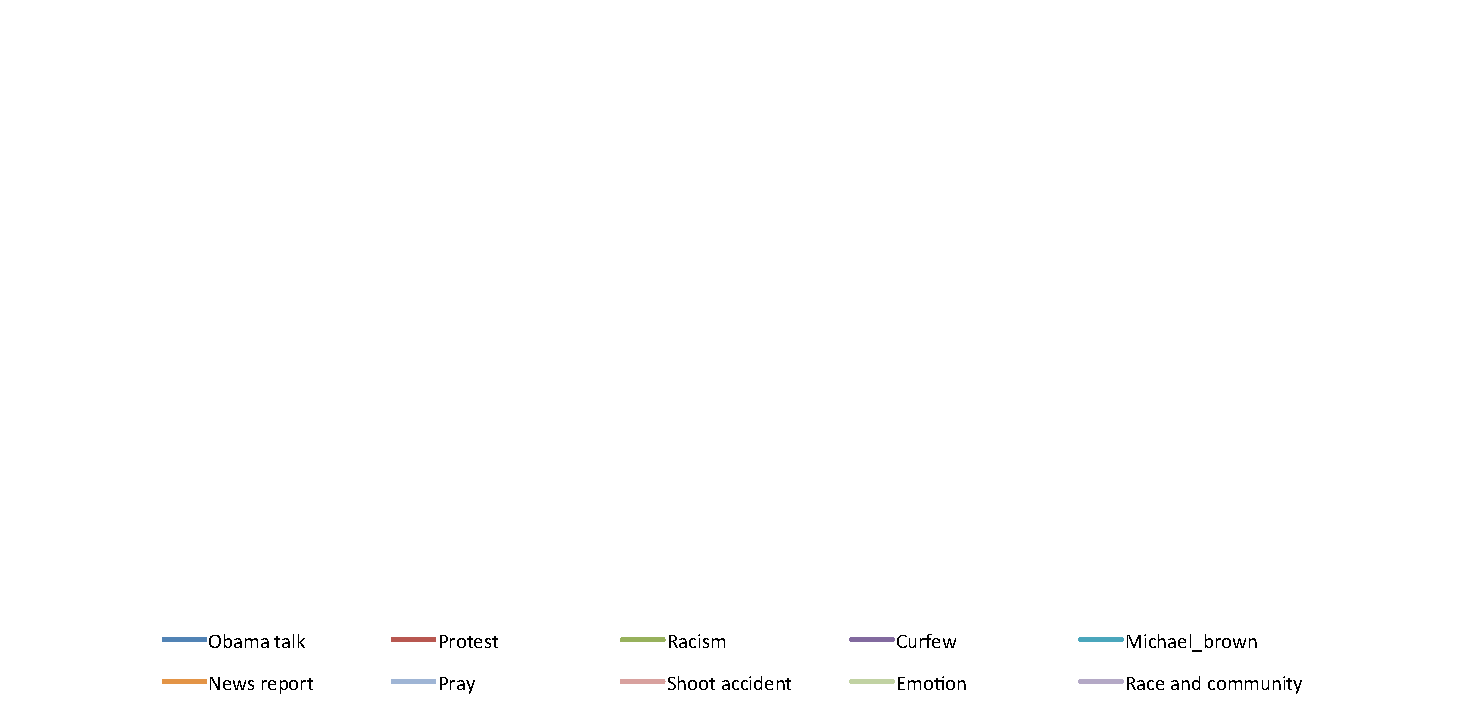
\includegraphics[width=\linewidth]{figures/Legend.pdf}
\caption{Tweets Topic Dynamics in and out of \stlouis by \stlda}\label{fig:tweets_topics_stlouis}
\end{figure*}

The proportion of tweets talking about \emph{Curfew} increases to 7.5\%, which is a peak on August 18 and then decreases. This topic change is similar for both tweets in and out of \stlouis area. Meanwhile the proportion of tweets talking about \emph{News Report} and \emph{Michael Brown} are similar along the time. Tweets about \emph{News Report} keep taking about 10\% to 15\% of all tweets. There are three small peaks on August 12, 14 and 22. Proportion of tweets talking about \emph{Michael Brown} and emph{Shoot Accident} increases a lot on August 15 in and out Ferguson area. It may be caused by the release of video recording Brown in a robbery prior to being shot. The public, both in and out of Ferguson area can be affected by it and begin to discuss a lot about it.

Difference lies in topic proportion of \emph{Pray}, but they share similar dynamics. Both in and out of \stlouis area, the increase of tweets with \emph{Pray} topic is consistent with the time when Michael Brown's funeral is held. On August 25, more than 35\% of tweets in Ferguson are about \emph{Pray}. Out of \stlouis, the number of tweets about \emph{Pray} increases to a peak on that day, taking 20\% of all.

It is reasonable to find that more tweets in \stlouis talk about \emph{Protest}, while out of \stlouis more tweets talk about \emph{Racism}. From August 18, when Governor Nixon deployed the National Guard to Ferguson, to August 21 when the National Guard withdrew, protests and conflicts keep occurring. People in Ferguson area are closer and more related to protests, so tweets with this topic surge to take more than 25\% of all tweets. Meanwhile proportion of \emph{Protest} tweets out of \stlouis is far less. The public who are not involved in the event tend to have less knowledge about real situations, but according to what they hear and know, they are better at abstract thinking about this event, thus \emph{Racism} takes majority in most of the time.

An interesting phenomenon is the \emph{Emotion} topic change. Michael Brown was killed on August 9, and anger emotion is the major topic of tweets in \stlouis, then \emph{Emotion} tweets keep decreasing, taking 10\% to 15\% of all tweets. However outside \stlouis area, there is a lag effect of \emph{Emotion} explosion. It is possible that news takes time to spread and the public outside Ferguson need more information to understand what happened. Besides, outsiders may care more about the conflicts between protesters and police, so their emotion was detonated when protests began.

Comparison of topic dynamics in and out of \stlouis area shows that, the public in \stlouis tends to publish tweets that are more related with evlovement of event, such as the shooting, protests and funeral. Meanwhile people out of \stlouis area has lag effect in \emph{Emotion} explosion and have more abstract perception on events, thus \emph{Racism} tweets take a majority. They share similar amount of focus on \emph{News Reports}, investigation of \emph{Michael Brown Shooting Accident} and \emph{Curfew}, which might because these issues are not quite closely related to them, or the influence is relatively small.

\subsection{Are Topic Dynamics of Tweets Similar with News?}

Using the results of \stlda, we compare the topics of news and tweets both in and out of \stlouis area. We observe that the three main topics in news, \emph{Obama Talk}, \emph{Shoot Accident} and \emph{Race and Community}, do not exist in tweets. However corresponding to shoot accident investigation, there is similar topic \emph{Michael Brown}, which is a main topic in tweets, taking a small proportion in news. Although the thing news and tweets talk about is the same, how they talk and what words they use is quite different, so it is identified with two separate topics for news and tweets. Similarly, \emph{Racism} topic exists mostly in tweets, while \emph{Race and Community} mainly exists in news. Although these two topics are talking about race, there is little overlapping of tweets and news in the two topics. It indicates that media and the public are using quite different words to discuss the same thing. One possible reason is that tweets use more oral language, while news uses more formal written language. It is also possible that media and the public describe the same thing with different frames. According to the top words in two topics, there are more negative words in \emph{Racism} such as \emph{stop}, \emph{riot}. In the topic labeled with \emph{Race and Community}, words like \emph{make}, \emph{good}, \emph{community} are indicative of positive emotion. Thus the public tends to have negative emotion about race issues during the Ferguson unrest, but the media tried to describe and lead the discussion to a positive way.

Two topics in tweets have little proportion in news, which are \emph{Emotion} and \emph{Prays}. It is reasonable that tweets are more subjective and contain more words about feelings, emotions and prays, while news is more serious and should be objective, avoiding emotional leadings. So the topic difference in tweets and news reflects the characteristics of two types of documents.

Another difference in news and tweets is topic diversity. Comparing topic dynamics of news (Figure~\ref{fig:news_topics_stlda}) and that of tweets (Figure~\ref{fig:tweets_topics_stlda}), it is obvious that tweets have more diverse topics, and proportion of different topics changes overtime. But there are only three main themes in news, and the changing of topics is rare. Topic related with Obama keeps a stable proportion in news report, while the report of investigation, and discussion of race issues keeps alternating dominance. The results show that public topics change along with evolvement of events, while media has certain issues to cover. Public opinions are more diverse. Under certain issues, voice of certain topic could become mainstream.

In general, the influence of media on the public is not obvious according to topic dynamics of news and tweets. Although they both concern with shoot accident and racism issues, how they talk is different. Besides there is not much similarity between topic dynamics of the two, even considering time lag. News have mainstream topics, but topics in tweets are more diverse, and evolve along with development of the event. The media care more about investigation of the shoot accident, reaction of the government and discussion of racism, but less about protests and emotion of the public. To large extent, the results support the theory of cascade model by ~\newcite{entman1993framing} from the perspective of the role media play, however the public do not shown to be heavily influenced by media frames. 

\subsection{Relation between Topic Dynamics of Tweets and News}
Meanwhile we examine the common topics in news and tweets to see whether there is interaction between news and tweets. Although the common topics take a small proportion in both news and tweets. The overlapping topics are \emph{Protest}, \emph{Curfew}, \emph{Michael Brown} and \emph{News Report}, which are shown in Figure~\ref{fig:topics_news_tweets}. We compare dynamics of these topics for news and tweets separately in and out of \stlouis area. For better observation of trend, we use smoothed line here instead of linear connection between points. The topic dynamic shapes for \emph{Protest} of news and tweets seem to be similar. \emph{Protest} has peaks on almost the same day for three sets of document, while \emph{Curfew} peak in news seems to have a slight lag after tweets. It is possible that people in Ferguson are under curfew and reporting it timely, but news may take some time to process information and publish.

\begin{figure*}[htpb]
\centering
\subfigure[Protest]
{
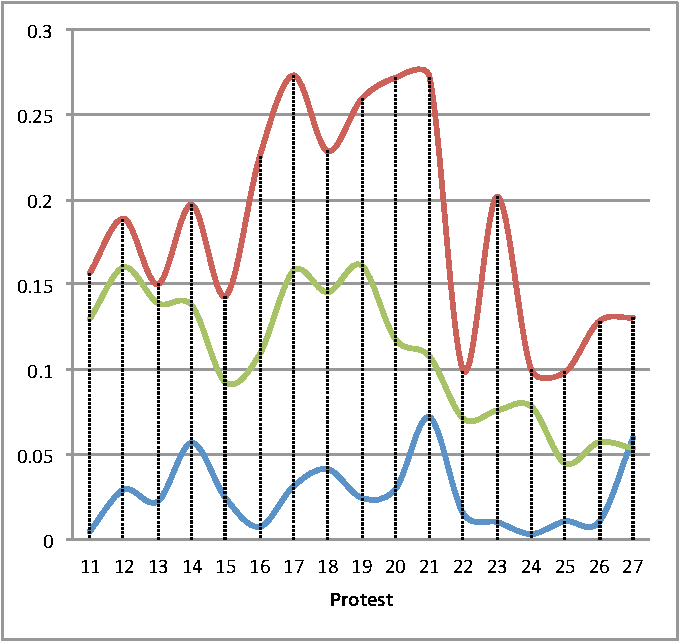
\includegraphics[width=0.48\linewidth]{figures/4_1_Protest.pdf}
\label{fig:protest}
}
\subfigure[Curfew]
{
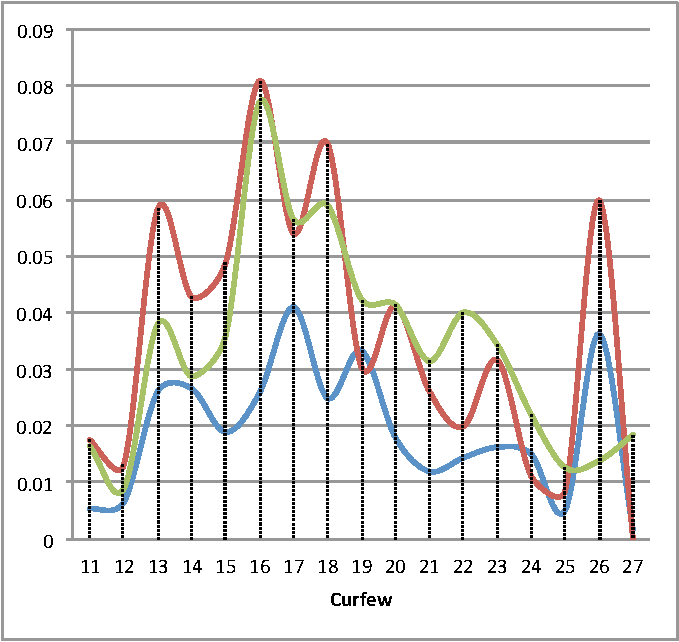
\includegraphics[width=0.48\linewidth]{figures/4_2_Curfew.pdf}
\label{fig:curfew}
}
\subfigure[Michael Brown]
{
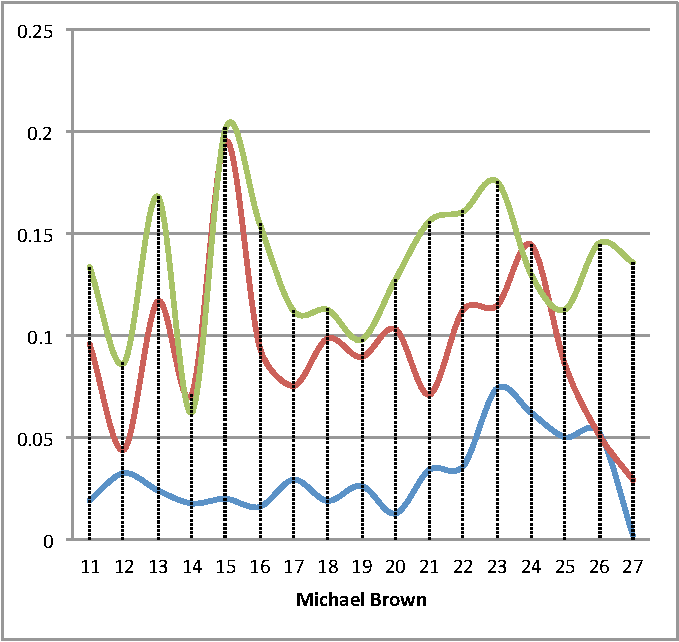
\includegraphics[width=0.48\linewidth]{figures/4_3_Michael_Brown.pdf}
\label{fig:mb}
}
\subfigure[News Report]
{
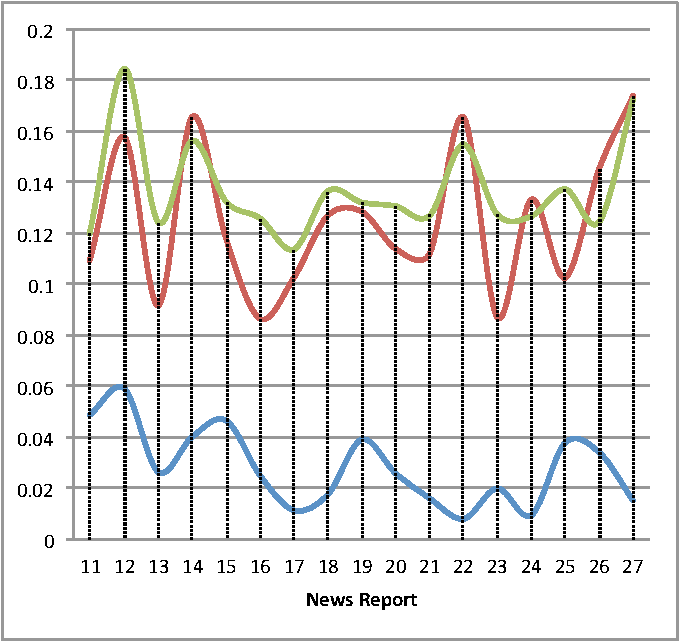
\includegraphics[width=0.48\linewidth]{figures/4_4_News_report.pdf}
\label{fig:news_report}
}
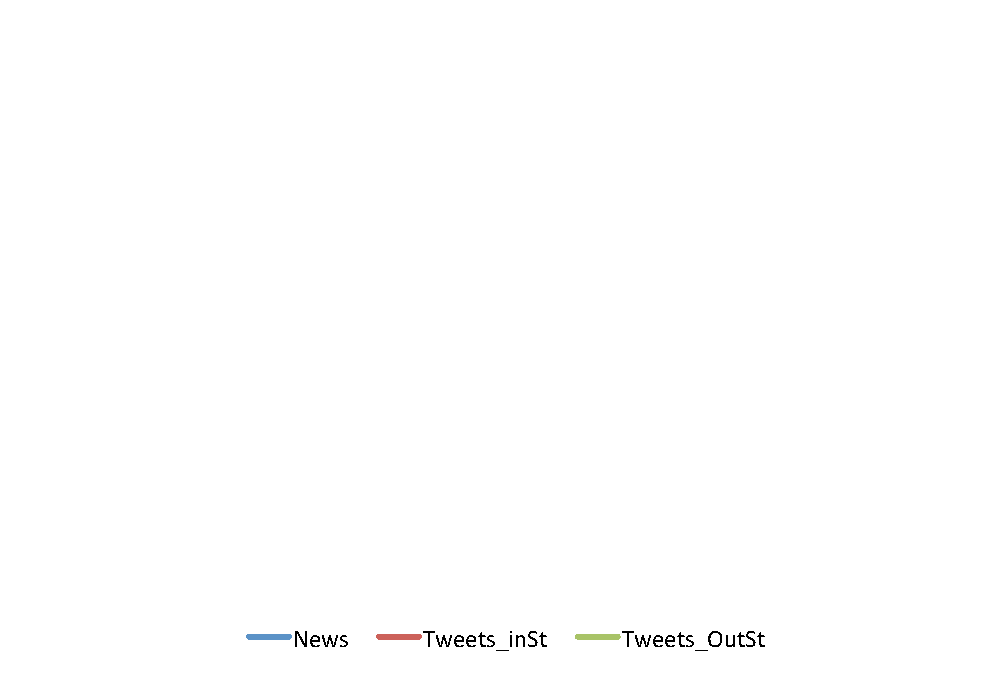
\includegraphics[width=0.5\linewidth]{figures/4_Legend_cut.pdf}
\caption{Topic Dynamic of News and Tweets by \stlda}\label{fig:topics_news_tweets}
\end{figure*}

There is no common pattern in \emph{Michael Brown}. According to analysis above, news mainly focus on investigation and getting to the bottom of shoot accident, which is labeled \emph{Shoot Accident}. It is talking about the same thing as topic \emph{Michael Brown}, however the words they use are quite different. So \emph{Michael Brown} topic has a tiny proportion in news, which takes less than 5\%.

For the topic \emph{News Report}, there is time difference in peaks of topic for news and tweets. However it is hard to know whether tweets cite some report first, and media is influenced to cite report, or in the other way around, or there may be no relation at all.